 \section{Поиск морфологических признаков по аналогии} \label{sect_exp_search_by_analog}
 В этом разделы описываются эксперименты по реализации алгоритмов определения части речи и грамсета по конечным буквосочетаниям, псевдоокончаниям.
 
 \subsection{Подготовка данных}
Для поиска части речи было сформировано множество из \emph{всех} лемм и словоформ морфологического словаря ВепКар. 
В этом множестве содержатся уникальные пары: слово — часть речи.

Для поиска грамсета было сформировано множество из (1) неизменяемых лемм (наречия, предлоги и т.д.) и (2) словоформ изменяемых частей речи. 
В этом множестве содержатся  уникальные пары: слово — грамсет. Для неизменяемых лемм грамсет равен $\O$.

Для обоих множеств вводим ограничения: слова должны состоять из более чем двух символов и не должны содержать пробельные символы. 
То есть аналитические формы и словосочетания были исключены из входных данных (См. раздел ~\ref{subsection:corpus_peculiarities}).  

\subsection{Поиск части речи по конечным буквосочетаниям (алгоритм POSGuess)}

Для оценки качества результата поиска по алгоритму POSGuess была предложена следующая функция $\text{eval}(\pos^u)$:

\begin{equation}\label{eq:metric-eval}
\text{eval} \left( 
    \begin{array}{@{}l@{\thinspace}l}
       \pos^u, \\
       \text{Counter} & \left[ \pos^k \right] \rightarrow c^k,\\
                      & \forall k = \overline{1,m} \\
    \end{array}
    \right)     = 
        \begin{cases}
            \multicolumn{2}{l}{\bluecomment{Массив Counter[\,] 
                  не содержит правильной
                  $\pos^u$.}}\\
            0, & \pos^u \ne \pos^k, \forall k = \overline{1,m},\\[3mm]
            \multicolumn{2}{l}{\bluecomment{\specialcell{Первые несколько POS могут иметь \\ 
                  одинаковые максимальные частоты $c^1$, \\
                  одна из этих POS совпадает с $\pos^u$.}}}\\
            1, & \pos^u \in \{ \left[ \pos^1, \ldots, \pos^j \right] : 
                               c^1=\ldots=c^j, j \leq m \},\\[4mm]
            \multicolumn{2}{l}{\frac{c^k}{ \sum_{k=1}^{m}c^k }, \; 
                \exists k : \pos^k = \pos^u, \;
                            c^k < c^1
                }
        \end{cases}
\end{equation}

Эта функция~(\ref{eq:metric-eval}) оценивает результат работы алгоритма POSGuess при условии, что нам известна правильная часть речи  $\pos^u$.

% Массив Counter, полученный с помощью алгоритма POSGuess, содержит частоты встречаемости слов для разных частей речи с тем же суффиксом, что и у исследуемого слова pos_u.
% Для каждой словоформы по алгоритму POSGuess определялся список частей речи, упорядоченный по числу похожих словоформ, имеющих ту же часть речи.
%
Алгоритм POSGuess считает количество слов, подобных слову  $u$ отдельно для каждой части речи и сохраняет результат в массив Counter, где ключами являются части речи, а значениями - количество слов этой части речи.
Массив Counter сортируется по значениям в убывающем порядке. Ключ первого элемента массива~--- часть речи с максимальным количеством слов, подобных несловарному слову $u$.

Для эксперимента были использованы \num{71 091} пара “слово - часть речи” для собственно карельского наречия и \num{399 260} пар “слово - часть речи” для вепсского языка. 

В ходе экспериментов были обнаружены два карельских слова, для которых не нашлось совпадений: ``cap'' (цап), ``štob'' (чтобы). 
%``cap'' (English: snap; Russian: \foreign{цап}) and the word ``štob'' (English: in order to; Russian: \foreign{чтобы}).
То есть в нашем словаре не нашлось других слов, оканчивающихся на -p и -b.
Такую уникальность окончаний можно объяснить тем, что эти два слова пришли в карельский язык из русского. 

Рисунок~\ref{fig:search_POS} показывает Соотношение вепсских (красная кривая) и карельских (синяя кривая) слов с правильной и неправильной частями речи, вычисленным алгоритмом POSGuess. 
Значения по оси X~--- значения функции $\text{eval}(\pos^u)$, 
см. формулу~(\ref{eq:metric-eval}). 
Эта функция для оценки присвоения части речи принимает следующие значения:

\begin{labeling}{eval-formula}
% Среди найденных частей речи отсутствует правильная у 4.7% вепсских слов и у 9% карельских слов (x=0 на рис.4).
\item [0] \num{4.7}\% вепсских слов и 9\% карельских слов ($x = 0$ на рис.~\ref{fig:search_POS}) была присвоена неправильная часть речи. 
Т.е., в результирующем массиве $Counter[\,]$ нет правильной части речи. 
Это первое условие в формуле~(\ref{eq:metric-eval}).
\hfill \break

\item [\num{0.1} -- \num{0.5}] 
\num{2.92}\% вепсских слов и \num{4.23}\% карельских слов ($x \in [0.1 ; 0.5]$ на рис.~\ref{fig:search_POS}) была частично присвоена правильная часть речи.
Т.е. массив $Counter[\,]$ содержит правильную часть речи, но она не в начале массива. 
Это последнее условие в формуле~(\ref{eq:metric-eval}).
\hfill \break

% Для 92.38% вепсских и 86.77% карельских слов получена оценка 1, т.е. правильная часть речи - на первом месте в списке найденных частей речи.
% Это второе значение в формуле (1).
\item [1] 
\num{92.38}\% вепсских слов и \num{86.77}\% карельских слов ($x = 1$ на рис.~\ref{fig:search_POS}) была присвоена правильная часть речи. 
Т.е. массив $Counter[\,]$ содержит правильную часть речи в начале массива. 
\end{labeling}

\begin{figure}
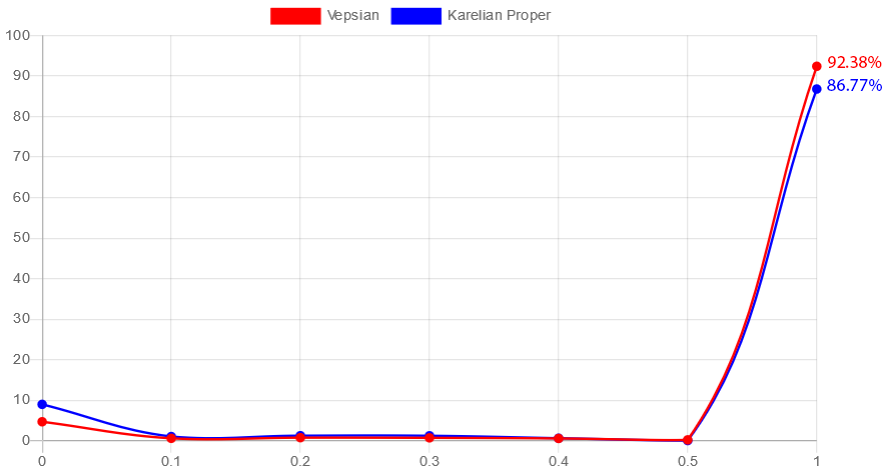
\includegraphics[width=1\textwidth]{experiments/pos_search_all_langs.png}
\caption{Соотношение вепсских (красная кривая) и карельских (синяя кривая) слов с правильной ($x=1$) и неправильной ($x=0$) частями речи, вычисленным алгоритмом POSGuess по формуле~(\ref{eq:metric-eval}).
} \label{fig:search_POS}
\end{figure}


Рисунок~\ref{fig:search_POS} показывает оценку результатов алгоритма POSGuess для всех частей речи в целом.
В таблицах ~\ref{tab:POS:quantity:Veps} (для вепсского языка) и Table~\ref{tab:POS:quantity:krl} (для карельского языка) представлена оценка тех же результатов работы алгоритма POSGuess, но для каждой части речи отдельно.

\begin{table}
% see example: http://dictorpus.krc.karelia.ru/en/experiments/results_search_pos?search_lang=1
\caption{Распределение оценок по частям речи для вепсских слов, 
%Number of Vepsian words of different parts of speech 
использованных в эксперименте.
Оценка результатов алгоритма POSGuess по формуле~(\ref{eq:metric-eval}) 
и доля слов в процентах, где столбец~\textit{0} означает долю слов с неправильной частью речью, \textit{1}~---  доля слов с правильной частью речью в начале списка, сгенерированного алгоритмом.}\label{tab:POS:quantity:Veps}

% The space between the text and the left/right border of its
\setlength{\tabcolsep}{8pt}

\begin{tabular}{ l r r r r r r r >{\bfseries}r } \toprule
     %&       &
     \multicolumn{2}{c}{\large вепсский} &
     \multicolumn{7}{c}{\specialcell{доля неугаданных (столбец 0), частично \\
     угаданных (0.1--0.5) и угаданных (1) POS, \%}} \\ \cmidrule(r){3-9}
                                                 % centering 1
 POS & Слова & 0 & 0.1 & 0.2 & 0.3 & 0.4 & 0.5 & \multicolumn{1}{c}{1}\\ \midrule
глагол & \num{93 047} & 2.12 & 0.52 & 0.55 & 0.47 & 0.36 & 0.01 & 95.97\\
сущ. & \num{240 513} & 2.88 & 0.3 & 0.67 & 0.6 & 0.42 & 0.24 & 94.89\\
прил. & \num{61 845} & 12.45 & 1.62 & 1.44 & 1.53 & 1.58 & 0.51 & 80.87\\
местоим. & \num{1 244} & 46.54 & 8.12 & 0.56 & 0.64 & 0 & 0 & 44.13\\
числ. & \num{1 200} & 44 & 6.25 & 2.33 & 0.67 & 0.33 & 0 & 46.42\\
наречие & 650 & 64.92 & 3.08 & 2.46 & 1.23 & 0.46 & 0 & 27.85\\
\bottomrule
\end{tabular}
\end{table}

\begin{table}
\caption{Распределение оценок по частям речи для карельских слов,
%Number of Karelian words of different parts of speech used in the experiment.
использованных в эксперименте.}\label{tab:POS:quantity:krl}

% The space between the text and the left/right border of its
\setlength{\tabcolsep}{8pt}

\begin{tabular}{ l r r r r r r r >{\bfseries}r } \toprule
     %&       &
     \multicolumn{2}{c}{\large карельский} &
     \multicolumn{7}{c}{\specialcell{доля неугаданных (столбец 0), частично \\
     угаданных (0.1--0.5) и угаданных (1) POS, \%}} \\ \cmidrule(r){3-9}
                                                 % centering 1
 POS & Слова & 0 & 0.1 & 0.2 & 0.3 & 0.4 & 0.5 & \multicolumn{1}{c}{1}\\ \midrule
глагол & \num{26 033} & 3.26 & 0.5 & 0.74 & 0.6 & 0.23 & 0.01 & 94.67\\
сущ. & \num{36 908} & 5.47 & 0.38 & 1.13 & 1.08 & 0.52 & 0.04 & 91.38\\
прил. & \num{6 596} & 35.81 & 6.66 & 4.15 & 4.56 & 2.73 & 0.38 & 45.71\\
местоим. & 610 & 81.64 & 2.13 & 0.66 & 3.11 & 2.3 & 0 & 10.16\\
числ. & 582 & 65.81 & 1.72 & 1.03 & 0.17 & 1.03 & 0 & 30.24\\
наречие & 235 & 68.51 & 3.4 & 2.98 & 2.13 & 0 & 0 & 22.98\\
\bottomrule
\end{tabular}
\end{table}

\begin{figure}
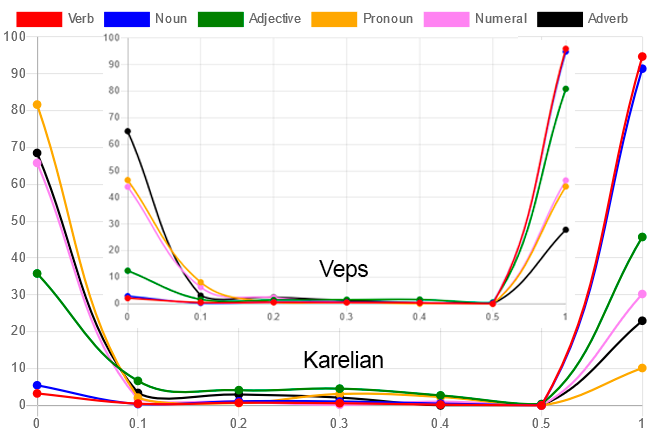
\includegraphics[width=1\textwidth]{experiments/POSdistrib.png}
\caption{Распределение оценок по частям речи для вепсских и карельских слов, использованных в эксперименте POSGuess.
%Number of Vepsian and Karelian words of different parts of speech used in the experiment.
} \label{fig:POS:distribution}
\end{figure}

 \subsection{Поиск грамсета по конечным буквосочетаниям (алгоритм GramGuess) и по псевдоокончанию (алгоритм GramPseudoGuess)}

Для оценки алгоритмов GramGuess и GramPseudoGuess были использованы \num{73 395} пар <<слово - грамсет>> для собственно карельского наречия и  \num{452 790} пар <<слово - грамсет>> для вепсского языка. 

Для каждого слова определялся список грамсетов, упорядоченный по числу подобных словоформ, имеющих тот же грамсет.

Для оценки качества результатов поисковых алгоритмов была предложена следующая функция $\text{eval}(g^u)$:
\begin{equation}\label{eq:metric-eval-gram}
\text{eval} \left( 
    \begin{array}{@{}l@{\thinspace}l}
       g^u, \\
       \text{Counter} & \left[ g^k \right] \rightarrow c^k,\\
                      & \forall k = \overline{1,m} \\
    \end{array}
    \right)     = 
        \begin{cases}
            \multicolumn{2}{l}{\bluecomment{Массив Counter[\,] 
                  не содержит правильного грамсета $g^u$.}}\\
            0, & g^u \ne g^k, \forall k = \overline{1,m},\\[3mm]
            \multicolumn{2}{l}{\bluecomment{\specialcell{Первые несколько грамсетов в массиве могут иметь \\ 
                  одинаковую максимальную частоту $c^1$, \\
                  один из этих грамсетов совпадает с $g^u$.}}}\\
            1, & g^u \in \{ \left[ g^1, \ldots, g^j \right] : 
                               c^1=\ldots=c^j, j \leq m \},\\[4mm]
            \multicolumn{2}{l}{\frac{c^k}{ \sum_{k=1}^{m}c^k }, \; 
                \exists \, k : g^k = g^u, \;
                            c^k < c^1
                }
        \end{cases}
\end{equation}

Эта функция~(\ref{eq:metric-eval-gram}) оценивает результаты алгоритмов GramGuess и GramPseudoGuess при условии, что нам известен правильный грамсет $g^u$.

\begin{table}
	\caption{Оценка результатов поиска грамсета для вепсского и карельского языков по алгоритмам GramGuess и GramPseudoGuess.}	
	\label{tab:Gram:quantity}

% The space between the text and the left/right border of its
\setlength{\tabcolsep}{8pt}

\begin{tabular}{ c c c c c} \toprule
     & \multicolumn{2}{c}{GramGuess}& \multicolumn{2}{c}{GramPseudoGuess}\\ \cmidrule(r){2-5}
%     &       GramGuess & & GramPseudoGuess & \\ \cmidrule(r){2-5}     
                                                
 Оценка & вепсский & карельский & вепсский & карельский\\ \midrule
0 & 2.53 & 5.72 & 7.9 & 9.23\\
0.1 & 0.53 & 0.83 & 1.04 & 1.57\\
0.2 & 0.71 & 1.16 & 1.24 & 1.37\\
0.3 & 0.64 & 0.89 & 2.68 & 1.36\\
0.4 & 0.2 &	0.56 & 0.14 & 0.68\\
0.5 & 0.11 & 0.09 & 0.83 & 0.43\\
1 &	\textbf{95.29} & \textbf{90.74} & \textbf{86.17} & \textbf{85.36}\\
\bottomrule
\end{tabular}
\end{table}

В таблице 4 видно, что алгоритм GramGuess показал себя лучше, чем GramPseudoGuess, а именно: 

\begin{labeling}{eval-formula}
% Среди найденных частей речи отсутствует правильная у 4.7% вепсских слов и у 9% карельских слов (x=0 на рис.4).
\item [карельский] 
%90.7\% versus 85.4\% for Karelian and 95.3\% versus 85.4\% for Veps.
90.7\% карельским словам был присвоен правильный грамсет по алгоритму GramGuess против 85.4\% по алгоритму GramPseudoGuess;
\hfill \break

\item [вепсский] 
95.3\% вепсским словам был присвоен правильный грамсет по алгоритму GramGuess против 85.4\% по алгоритму GramPseudoGuess.
\end{labeling}

Возможно причина в том,  что конечные буквосочетания длиннее псевдоокончаний и дают больше информации. 
К тому же алгоритм GramPseudoGuess не подходит для частей речи без флективных форм.


\subsection{Анализ ошибок алгоритмов поиска по аналогии}

% TODO нарисовать картинку для третьего алгоритма, 
% где для неизвестного слова u
% поочерёдно подбираются существующие слова из словаря 
% со всё укорачивающимся псевдоокончанием...
Для анализа ошибок были взяты результаты работы алгоритма POSGuess и визуализированы с помощью программы Graphviz.
% Доля и число ошибок в определении части речи, визуализация с помощью инструмента Graphviz
%
%
% Построены графы ошибок перехода для определения части речи 
% алгоритмом POSGuess для вепсского (рис. 7а)
% fig:pos-error-graph-vep
% и собственно карельского наречия карельского языка (рис. 7б).
% fig:pos-error-graph-krl
%
Были построены графы ошибок перехода для определения части речи алгоритмом POSGuess для вепсского
(рис.~\ref{fig:pos-error-graph-vep}) и собственно карельского наречия карельского языка (рис.~\ref{fig:pos-error-graph-krl}).

Объясним, как этот граф построен.
% Рассмотрим на правом рисунке (рис. 7б) толстую зелёную вертикальную стрелку с метками 21.6%, 1424, 3.9%, соединяющую прилагательные и существительные.
Например, толстая серая вертикальная стрелка соединяет прилагательные и существительные (рис.~\ref{fig:pos-error-graph-krl}), и эта стрелка имеет метки 21.6\%, 1424 and 3.9\%. 
Это означает, что алгоритм POSGuess ошибочно определил 1424 карельских прилагательных как существительные. 
Это составило 21.6\% от всех карельских прилагательных и 3.9\% от существительных.
Это можно объяснить тем, что
одна и та же лемма (в вепсском и карельском) может выступать в роли существительно и прилагательного. 
То есть в обоих языках есть одинаковые леммы для существительных и прилагательных.
Они и склоняются одинаково.

Эксперимент показал, что в нашей выборке таких лемм для собственно 
карельского языка существенно больше, чем для вепсского языка 
(21.6\% против 9.8\% на рис.~\ref{fig:pos-error-graph}). 
Хотя в абсолютных числах вепсский превышает карельский, а именно: 
6061 против 1424 ошибок такого рода. Это объясняется большим размером вепсского словаря в ВепКар.

\begin{figure}
\centering
\begin{subfigure}{.5\textwidth}
  \centering
  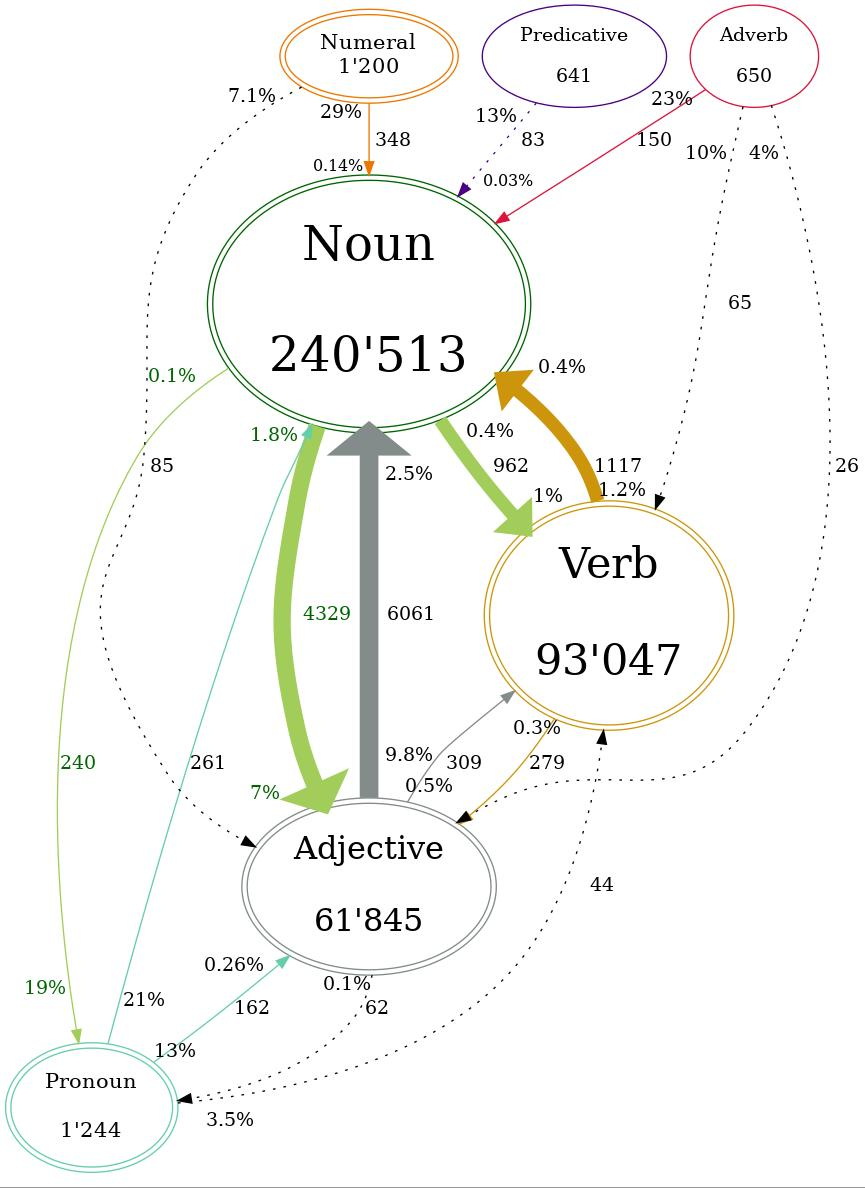
\includegraphics[width=0.95\textwidth]{experiments/247_veps_only_max0_pos-1_0.jpg}
  \caption{вепсский язык}
  \label{fig:pos-error-graph-vep}
\end{subfigure}%
\begin{subfigure}{.5\textwidth}
  \centering
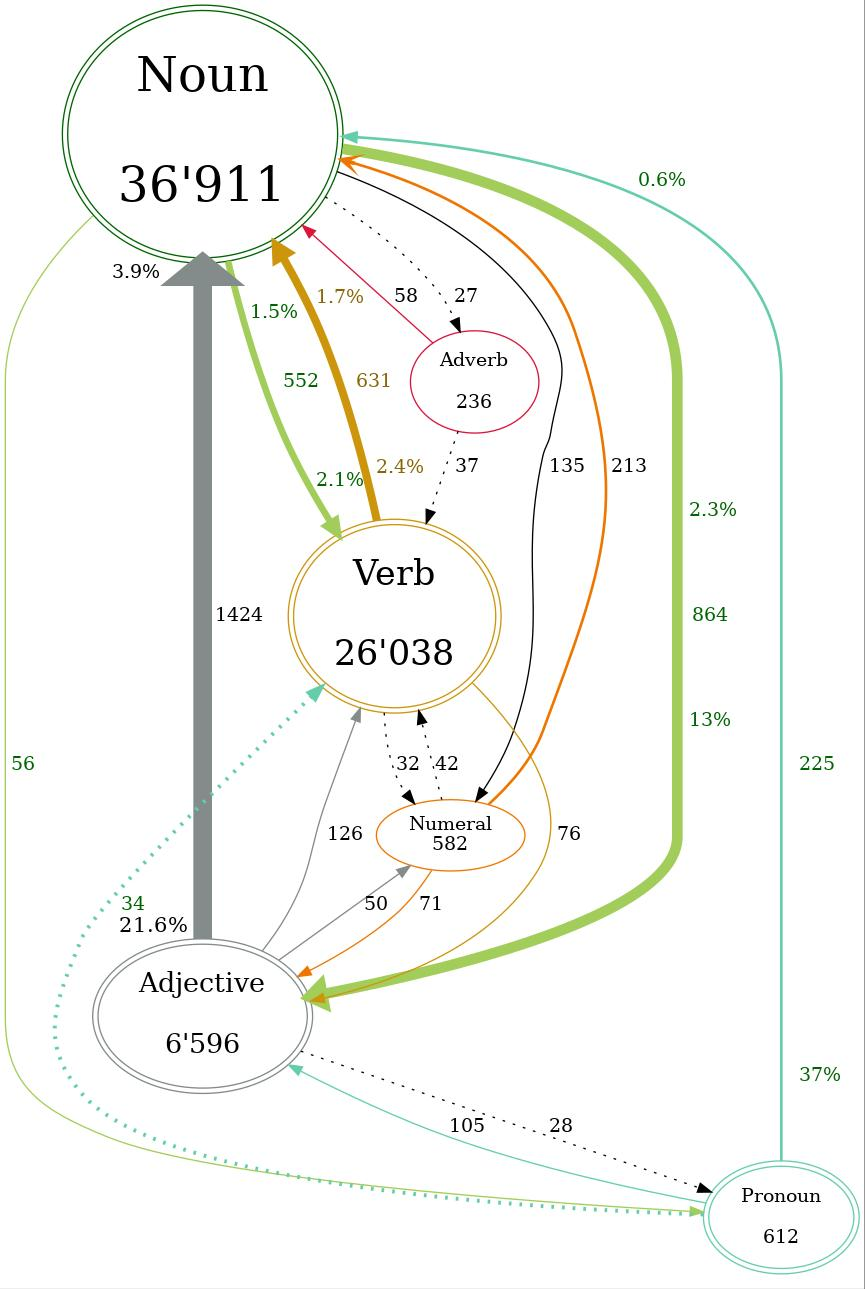
\includegraphics[width=1.0\textwidth]{experiments/456_pos-4_20_number-krl.jpg}  \caption{собственно карельское наречие карельского языка}
  \label{fig:pos-error-graph-krl}
\end{subfigure}
\caption{Граф перехода ошибок поиска части речи, который отражает результаты алгоритма POSGuess. }
\label{fig:pos-error-graph}
\end{figure}
 
